% !TeX root = ../main.tex
\section{Исследование влияния квадратурного дисбаланса гетеродина на динамический диапазон}

В реальных радиотехнических трактах и цифровых смесителях ортогональность квадратурных каналов может нарушаться из-за наличия амплитудного ($\Delta A$) или фазового ($\Delta \varphi$) дисбаланса. Аналитически опорный сигнал гетеродина с учетом погрешностей описывается соотношением:
\begin{equation}
    g_{\text{дисб}}[n] = 10^{\frac{\Delta A}{20}} \cos(2\pi f_G n T_s) - j \sin(2\pi f_G n T_s + \Delta \varphi),
    \label{eq:nco_imbalance}
\end{equation}
где:
\begin{itemize}
    \item $\Delta A$ --- амплитудный дисбаланс квадратур в децибелах (параметр \texttt{amv});
    \item $\Delta \varphi$ --- фазовый дисбаланс (отклонение разности фаз квадратур от $90^\circ$, параметр \texttt{pmv});
    \item $f_G$ --- частота гетеродина ($210.0$ МГц);
    \item $T_s = 1/f_s$ --- период дискретизации входного тракта ($1/180$ МГц);
    \item $n$ --- номер временного отсчета.
\end{itemize}

Нарушение ортогональности каналов приводит к неполной взаимной компенсации побочных спектральных компонент при квадратурном переносе частоты. С ростом дисбаланса уровень этих составляющих увеличивается, что напрямую снижает величину SFDR.

На рисунке \ref{fig:sfdr_imbalance} приведены зависимости динамического диапазона SFDR от амплитудной и фазовой асимметрии каналов.

\begin{figure}[H]
    \centering
    \begin{minipage}{0.48\textwidth}
        \centering
        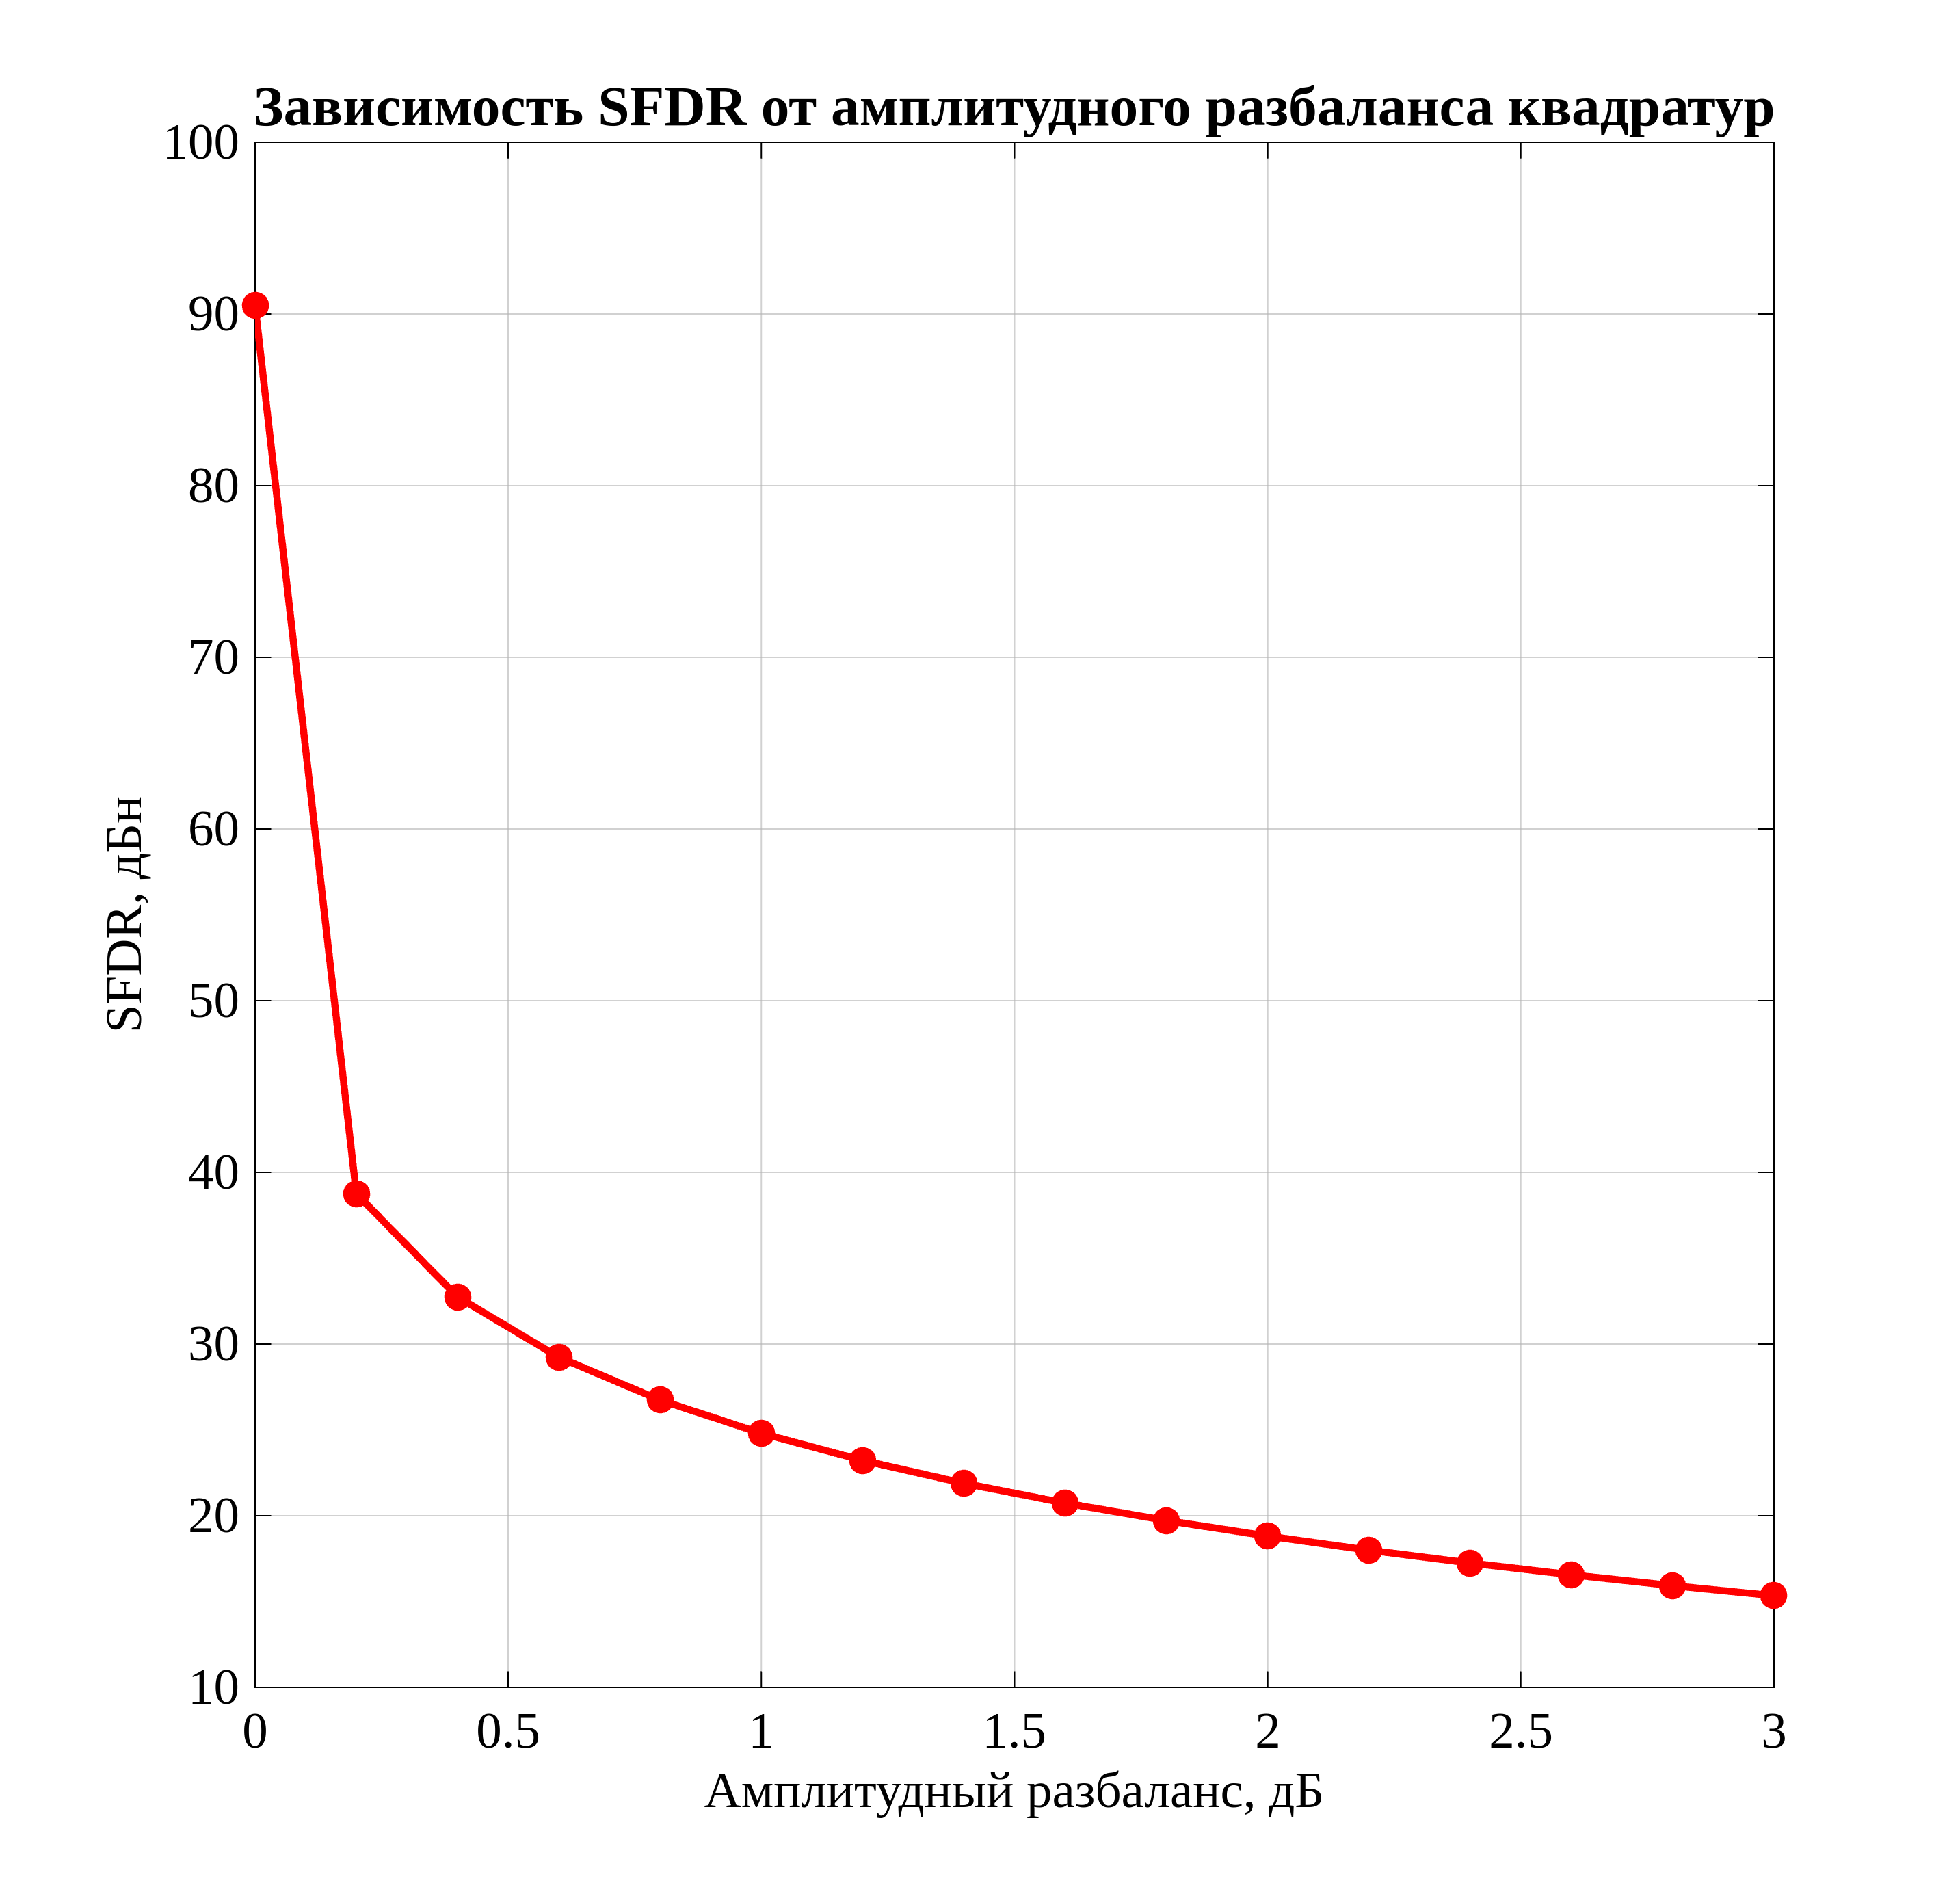
\includegraphics[width=\textwidth]{export_figs/p4_sfdr_vs_amv.png}
        \caption*{а) Зависимость от амплитудного дисбаланса}
    \end{minipage}\hfill
    \begin{minipage}{0.48\textwidth}
        \centering
        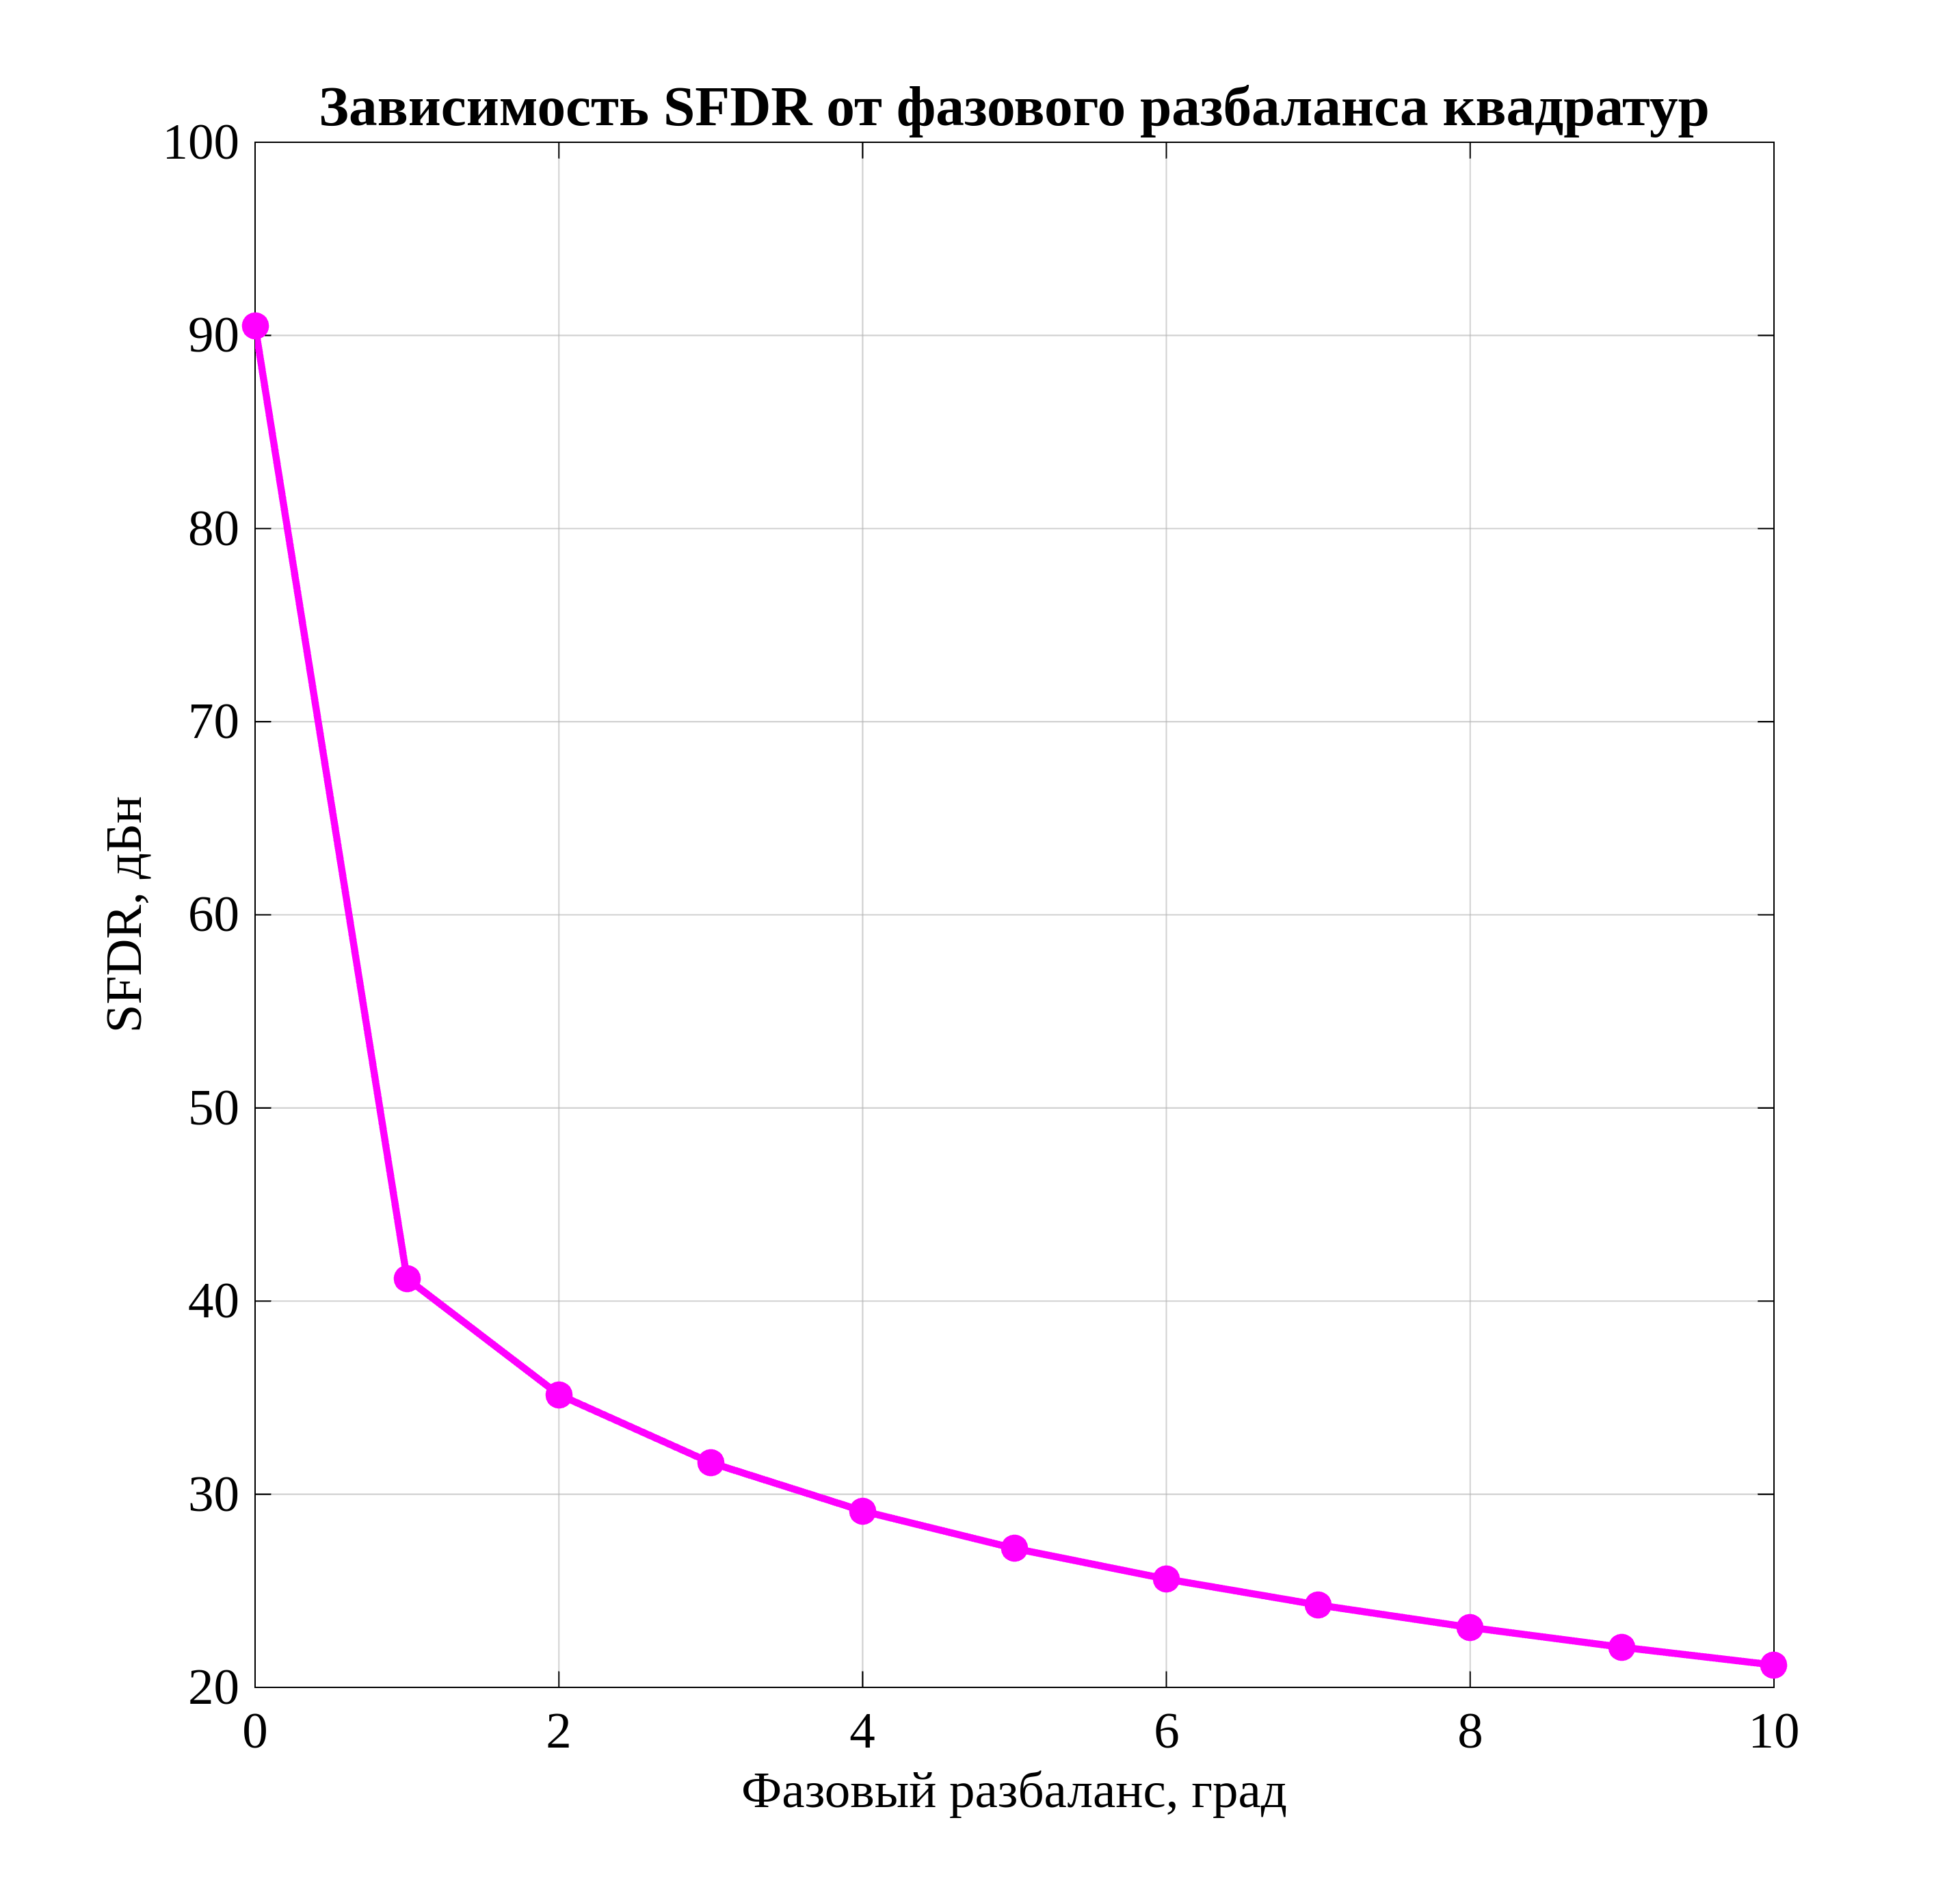
\includegraphics[width=\textwidth]{export_figs/p4_sfdr_vs_pmv.png}
        \caption*{б) Зависимость от фазового дисбаланса}
    \end{minipage}
    \caption{Зависимость динамического диапазона SFDR от параметров квадратурного дисбаланса гетеродина}
    \label{fig:sfdr_imbalance}
\end{figure}

Анализ полученных характеристик показывает:
\begin{enumerate}
    \item Максимальный динамический диапазон достигается при строгой ортогональности и балансе амплитуд ($\Delta A = 0\text{ дБ}$, $\Delta \varphi = 0^\circ$).
    \item Любое отклонение амплитуды или фазы приводит к резкой деградации SFDR из-за монотонного роста мощности неподавленных паразитных составляющих.
\end{enumerate}
